\documentclass[tikz,border=2pt]{standalone}
\usepackage{amsmath}
\usepackage{pgfplots}
\pgfplotsset{compat=1.18}
\usetikzlibrary{arrows.meta}
\begin{document}
% Player 1's payoffs (against L, against R): U=(3,0), M=(0,3), D=(1,1). Neither U nor M lies in
% the region {>1,>1} that beats D in both columns, but the mixture (1/2)U+(1/2)M=(1.5,1.5) does.
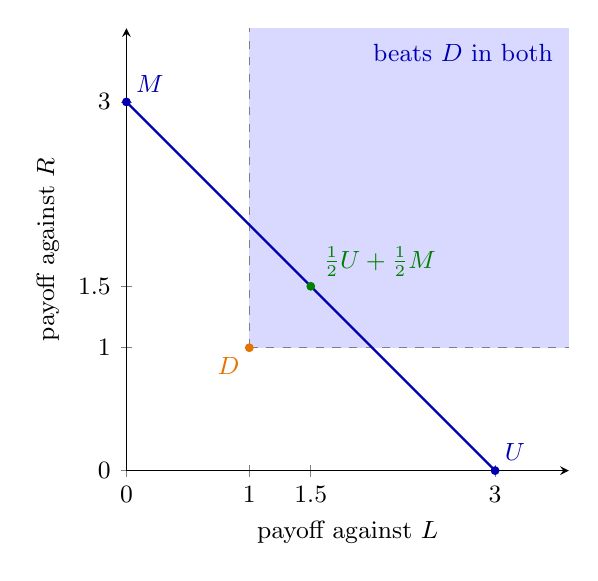
\begin{tikzpicture}[font=\small, >={Latex[length=2mm]}]
  \begin{axis}[width=7.2cm, height=7.2cm, axis lines=left,
      xmin=0, xmax=3.6, ymin=0, ymax=3.6,
      xtick={0,1,1.5,3}, ytick={0,1,1.5,3},
      xticklabels={$0$,$1$,$1.5$,$3$}, yticklabels={$0$,$1$,$1.5$,$3$},
      xlabel={payoff against $L$}, ylabel={payoff against $R$},
      clip=false]
    % strategies that strictly beat D in both columns
    \fill[blue!15] (axis cs:1,1) rectangle (axis cs:3.6,3.6);
    \draw[gray, dashed] (axis cs:1,1) -- (axis cs:1,3.6);
    \draw[gray, dashed] (axis cs:1,1) -- (axis cs:3.6,1);
    \node[blue!70!black, anchor=north east] at (axis cs:3.55,3.55) {beats $D$ in both};
    % mixtures of U and M
    \draw[thick, blue!70!black] (axis cs:3,0) -- (axis cs:0,3);
    \fill[blue!70!black] (axis cs:3,0) circle (1.6pt) node[above right] {$U$};
    \fill[blue!70!black] (axis cs:0,3) circle (1.6pt) node[above right] {$M$};
    \fill[green!50!black] (axis cs:1.5,1.5) circle (1.6pt)
      node[above right, xshift=1pt] {$\tfrac12U+\tfrac12M$};
    \fill[orange!90!black] (axis cs:1,1) circle (1.6pt) node[below left] {$D$};
  \end{axis}
\end{tikzpicture}
\end{document}
